Fox-Wolfram moments can be used to parametrise the momentum and energy flow distributions and were introduced in Ref.~\cite{Fox:1978vu}.
They are defined for a collection of momentum, $\vec{p}_i$, as:
\begin{equation}
    H_l \equiv \sum_{i,j} |\vec{p}_i||\vec{p}_j|P_l(\cos\theta_{ij}),
\end{equation}
where $\theta_{ij}$ is the angle between $p_i$ and $p_j$, and $P_l$ are the Legendre polynomials.
Normalised Fox-Wolfram moments,
\begin{equation}
R_l\equiv \frac{H_l}{H_0},
\end{equation}
are often used, as strongly collimated sets of momenta tend to zero for $l_{\mathrm{odd}}$ and to one for $l_{\mathrm{even}}$ \cite{BaBar:2014omp}.
Conventionally, $R_{1-4}$ are considered.
In addition, in this study, we calculate $R_2^B$, which only includes momenta of particles used for reconstruction of the tag-$B$ meson candidate.
The distributions for \textbf{Test~1} are shown in \Cref{fig:foxWolframR1,fig:foxWolframR2,fig:foxWolframR3,fig:foxWolframR4,fig:Btag_R2}.
All these observables prove to be strongly correlated with the photon energy spectrum.

\begin{figure}[htbp!]
    \subcaptionbox{\label{fig:foxWolframR1}}{
        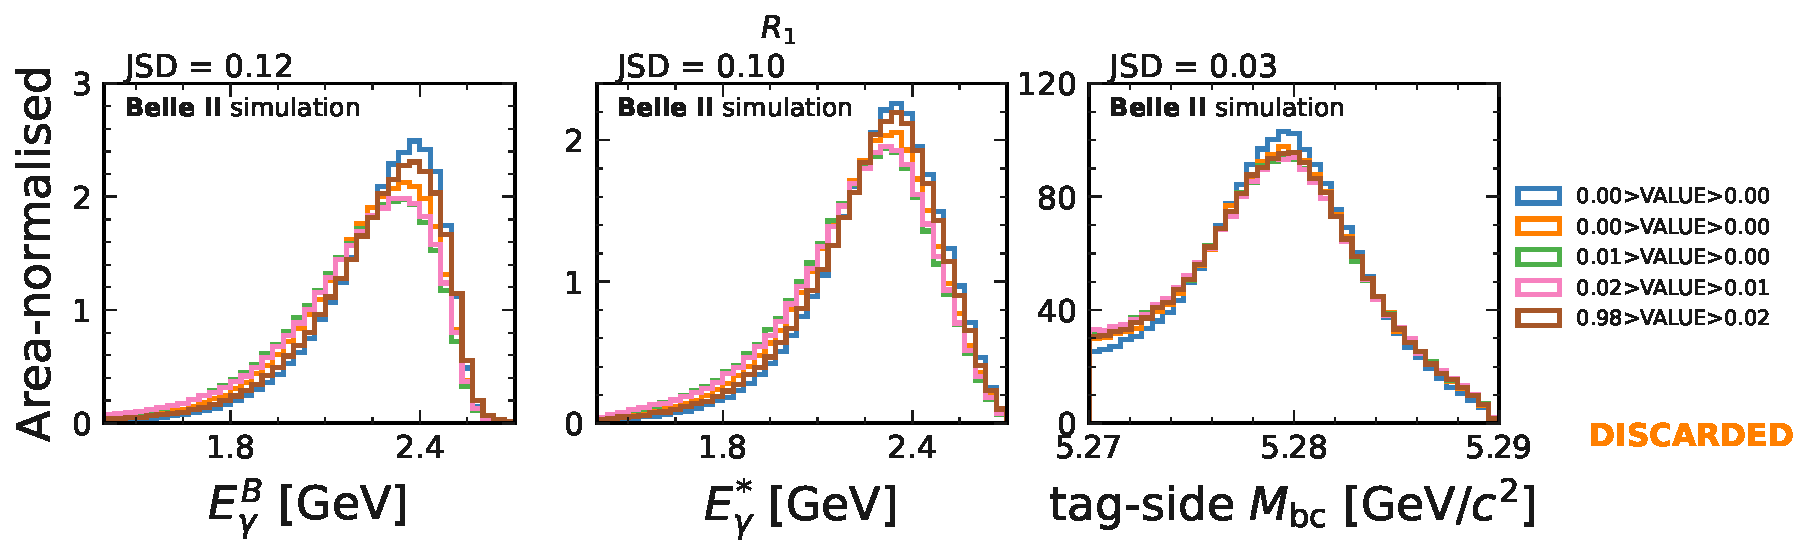
\includegraphics[width=0.95\textwidth]{figures/appendices/continuum_suppression_features/fox_wolfram_moments/foxWolframR1_bias_tested.pdf}
    }
    \subcaptionbox{\label{fig:foxWolframR2}}{
        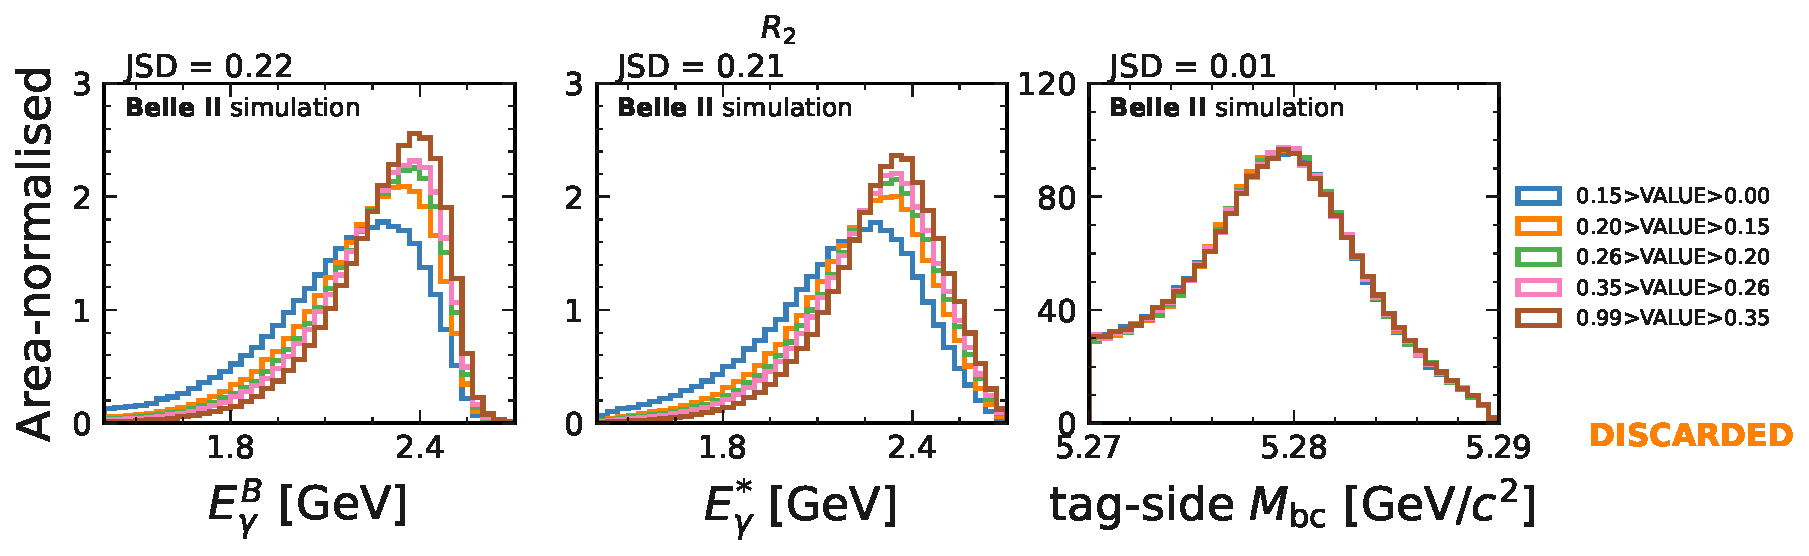
\includegraphics[width=0.95\textwidth]{figures/appendices/continuum_suppression_features/fox_wolfram_moments/foxWolframR2_bias_tested.pdf}

    }
\end{figure}
\begin{figure}[htbp!]
    \ContinuedFloat
    \subcaptionbox{\label{fig:foxWolframR3}}{
        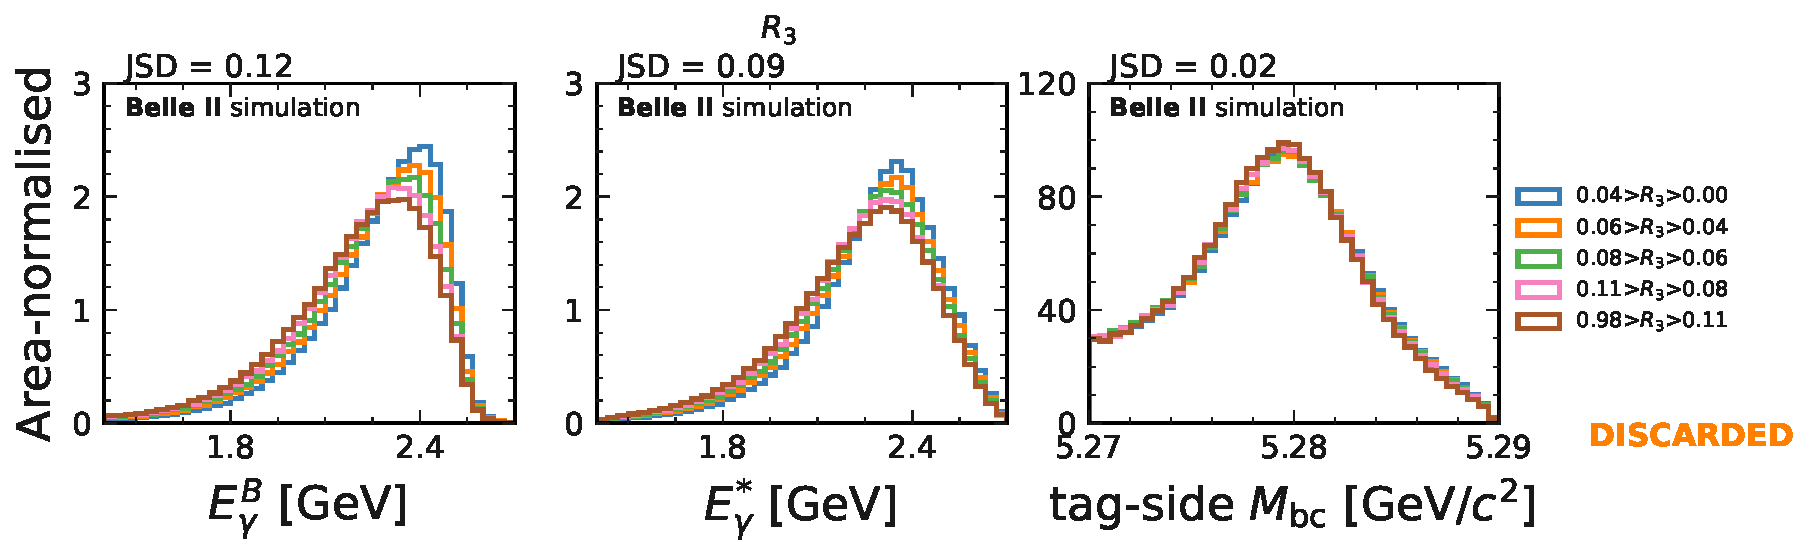
\includegraphics[width=0.95\textwidth]{figures/appendices/continuum_suppression_features/fox_wolfram_moments/foxWolframR3_bias_tested.pdf}

    }
    \subcaptionbox{\label{fig:foxWolframR4}}{
        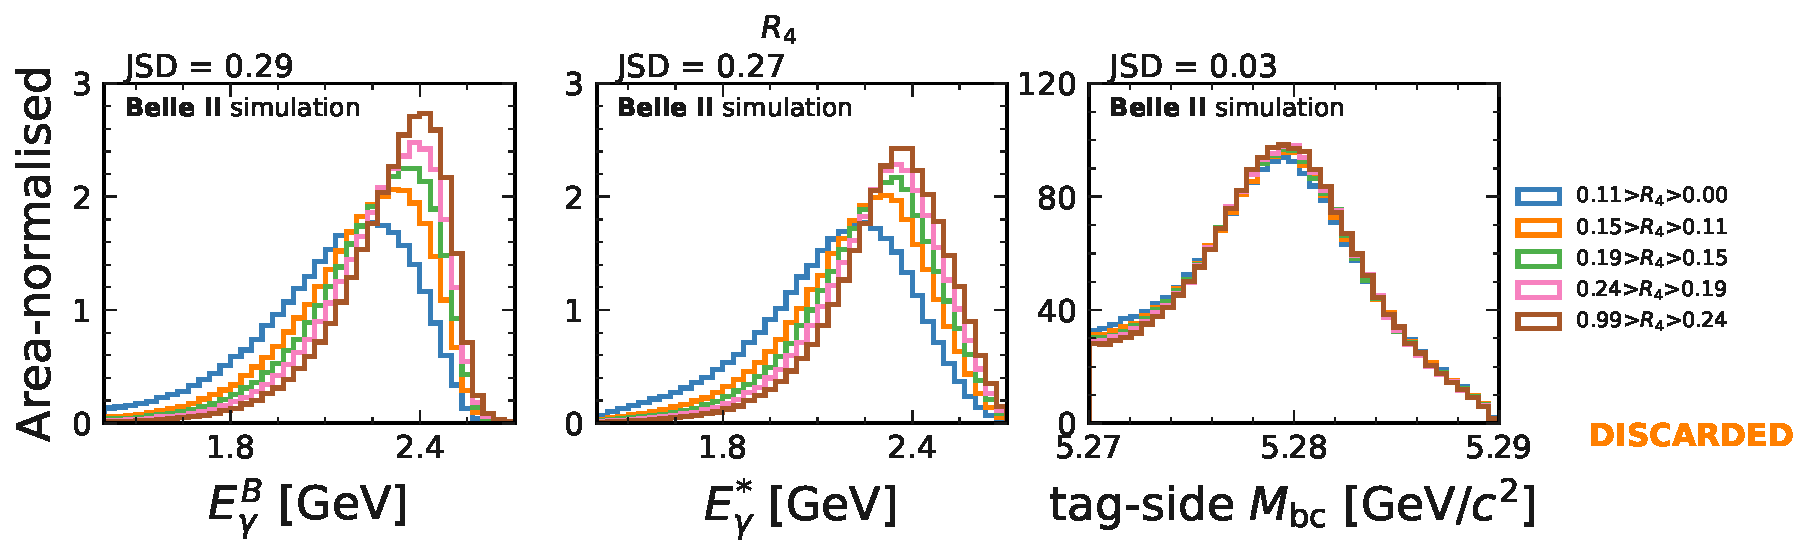
\includegraphics[width=0.95\textwidth]{figures/appendices/continuum_suppression_features/fox_wolfram_moments/foxWolframR4_bias_tested.pdf}

    }
    \subcaptionbox{\label{fig:Btag_R2}}{
        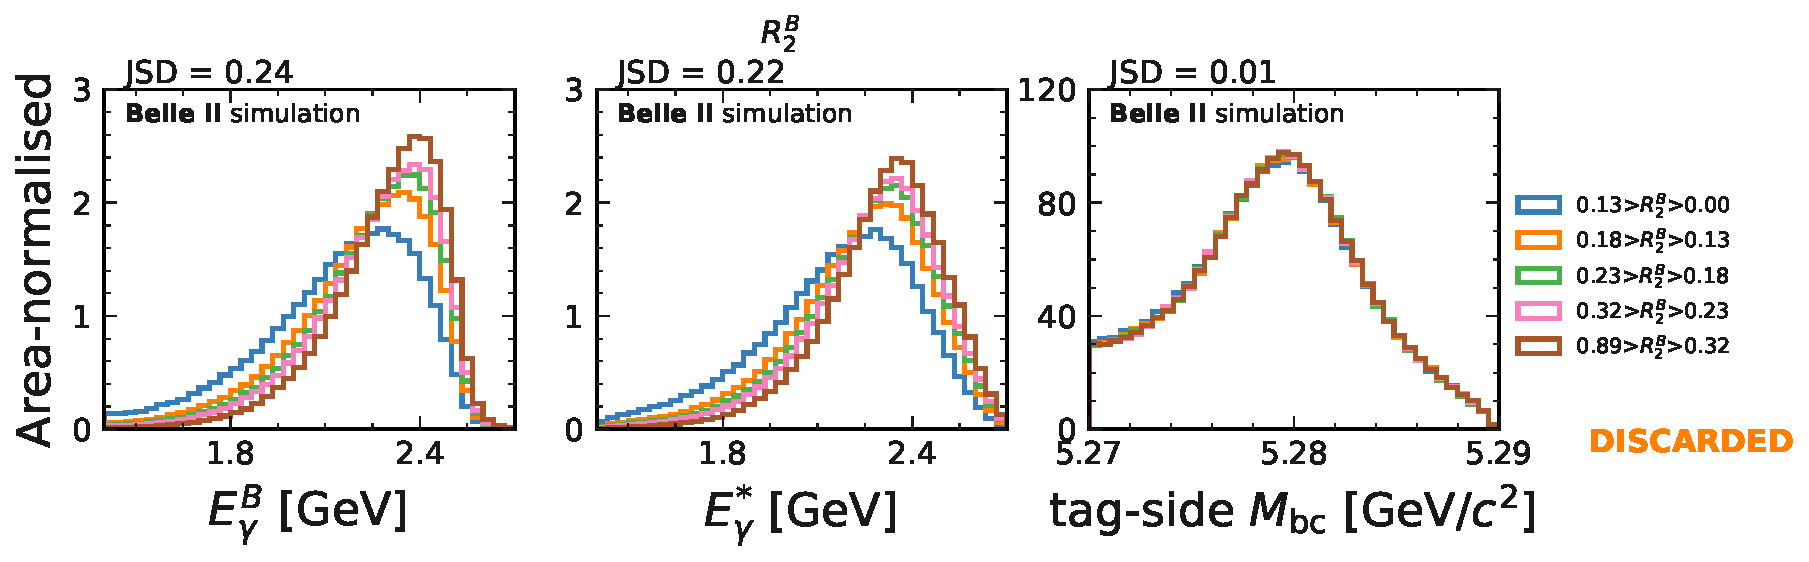
\includegraphics[width=0.95\textwidth]{figures/appendices/continuum_suppression_features/fox_wolfram_moments/Btag_R2_bias_tested.pdf}

    }
    \caption{\label{fig:fox_wolframs_test1} The bias-test on \EB, \Estar and \Mbc for Fox-Wolfram moments.
    The test is performed based on \textbf{Test~1} strategy, defined in \Cref{sec:continuum_features}.
    Variable definitions are given in the text.
    The Jensen Shannon distance as introduced in \Cref{eq:js_distance} is given for each distribution.
    }
\end{figure}
